\chapter{Lokale Kurventheorie im euklidischen Raum}
\section{Grundbegriffe der Kurventheorie}
Wir betrachten zunächst (kurzzeitig) rein \uline{affingeometrische} Begriffe/Invarianten.
\begin{definition}
 Ein \uline{\(\C^r\)-Weg}\index{Weg} oder eine \uline{parametrisierte \(\C^r\)-Kurve}\index{Kurve} (\(r\ge 0\)) [\(\C^r = r\)-mal stetig differenzierbar] im (affinen) \(\IR^n\) ist eine \(\C^r\)-Abbildung 
\[
 c: t\in I \subset \IR \mapsto c(t)\in \IR^n
\]
eines offenen Intervalls \(I\) in den \(\IR^n\). \\
\(t\) heißt \uline{Parameter}\index{Parameter}, die Bildmenge \(c[I] \subset \IR^n\) die \uline{Spur des Weges}\index{Spur}. \\
Ein \(\C^r\)-Weg (\(r\ge 1\)) heißt \uline{regulär}\index{regulär}, wenn überall der \uline{Tangentenvektor}\index{Tangentenvektor} \(\dot c(t) = \frac{\dd c}{\dd t}(t) \ne 0\) ist. Nichtreguläre Punkte \(c(t_0)\) mit \(\dot c(t_0)=0\) heißen \uline{Singularitäten}\index{Singularität}.
\end{definition}
\begin{kin}
\(t \mapsto c(t)\) beschreibt die \uline{zeit}abhängige Bewegung eines Punktes im \(\IR^n\).
\(\dot c\) ist die vektorielle Geschwindigkeit\index{Geschwindigkeit} (und im euklidischen \(\IR^n\) \(w:= | \dot c|\) die skalare Geschwindigkeit).
\end{kin}
\begin{bsp}\(\)
\begin{enumerate}
 \item \uline{Peano-Kurve}: Stetiger (\(\C^0\)-)Weg im \(\IR^2\), dessen Spur jeden Punkt eines Gebietes \(G\subseteq \IR^2\) ausfüllt (nirgends differenzierbar, "`unbrauchbar"')
 \item \uline{Konstanter Weg}: \(t \in I \mapsto c(t)=x_0 \in \IR^n\) (nirgends regulär, "`unbrauchbar"')
 \item \uline{Neil'sche Parabel}: \(c: t\in \IR \mapsto c(t) = \begin{pmatrix}
                                                                t^2 \\
								t^3
                                                               \end{pmatrix}
								\in \IR^2 \)\quad (\(\C^\infty\)-Weg), in \(c(0)=\begin{pmatrix}
								                                                  0 \\
														  0
								                                                 \end{pmatrix} \) nicht regulär ("`Spitze"') (\(w(0)=|\dot c (0)|=0\), "`man hat Zeit, sich umzudrehen"')
 \item \uline{Kreislinie}: \(c: t\in \IR \mapsto c(t)=\begin{pmatrix}
                                                       \cos t \\
						       \sin t
                                                      \end{pmatrix} \in \IR^2\) ( \(\infty\)-oft durchlaufbar) [Affin gesehen ist das eine Ellipse!] \\
Aber auch \(t \mapsto \tilde c(t) = \begin{pmatrix}
                                     t \\
				     \pm \sqrt{1-t^2}
                                    \end{pmatrix} \) und \(t \mapsto \tilde{\tilde c}(t)=\begin{pmatrix}
											  \frac{1}{\cosh t} \\
											  \tanh t
											 \end{pmatrix} \)
sind Parametrisierungen von Kreisstücken.
\end{enumerate}
\end{bsp}
Wege,  die nur mit veränderlicher "`Zeitskala"' durchlaufen werden, sollen nicht als verschieden angesehen werden.
\begin{definition}
 \(I, \tilde I \subset \IR\) seien offene Intervalle. \\
Zwei Wege \(c: I \to \IR^n, \tilde c: \tilde I \to \IR^n\) heißen \uline{\(C^r\)-äquivalent}\index{Äquivalenz} (\(r\ge 0 \)), wenn ein orientierungstreuer\index{orientierungstreu} (d.h. monoton wachsender) \(\C^r\)-Diffeomorphismus\index{Diffeomorphismus} \(\Phi : I \to \tilde I\) existiert, mit
\[
 \uline{c= \tilde c \circ \Phi}, \text{ d.h. } \uline{\forall_t c(t)=\tilde c (\Phi(t))}
\]

\end{definition}

\begin{bemerkung} \(\)
 \begin{enumerate}
  \item[0.] \(\Phi \, \C^r\)-Diffeomorphismus\index{Diffeomorphismus} \(\Leftrightarrow \Phi\) bijektiv und \(\Phi\) \uline{und \(\Phi^{-1}\)}\, \(C^r\)-differenzierbar. 
  [Bsp.: \(\Phi: t \in \IR \to t^3 \in \IR\) ist \uline{kein} \(\C^1\)-Diffeomorphismus] \\
  Bei \(C^r\)-Diffeomorphismus ist stets \(\dot \Phi(t)\ne 0\) (falls \(r\ge 1\))
  \item[1.] \(\Phi\) ist (für \(r\ge 1\)) genau dann orientierungstreu, wenn überall \(\dot \Phi(t)>0\) ist.
  \item[2.] Äquivalente Wege besitzen (für \(r\ge 1\)) das gleiche Regularitätsverhalten.
  \[
   \dot c(t)= \dot{\tilde c} (\Phi(t)) \cdot \underbrace{\dot \Phi(t)}_{>0}
  \]
  \item[3.] Die Äquivalenz von Wegen ist wirklich eine Äquivalenzrelation (reflexiv, symmetrisch, transitiv)
 \end{enumerate}
\end{bemerkung}

\begin{definition}
 Eine (orientierte, reguläre) \uline{\(\C^r\)-Kurve} (\(r\ge1\)) im (affinen) \(\IR^n\) ist eine Äquivalenz-klasse \([c]\) von regulären \(\C^r\)-Wegen \(c : I \subset \IR \to \IR^n\). Ein Repräsentant heißt eine (zulässige) \uline{Parametrisierungen}\index{Parametrisierung} der \(\C^r\)-Kurve, eine die Äquivalenz vermittelnde Abbildung \(\Phi\) eine (zulässige) \uline{Parametertransformation}\index{Parametertransformation}.
\end{definition}

\begin{bsp}
 Die "`Kreis"'-Darstellungen\index{Kreis} 
 \[
 t \mapsto c(t)=\begin{pmatrix}
                 \cos t \\
                 \sin t
                \end{pmatrix} \in \IR^2, \left(|t|<\frac\pi2\right)
 \]
 und 
     \[
      \tilde t\mapsto \tilde c(\tilde t) = \begin{pmatrix}
                                             \frac1{\cosh \tilde t} \\
                                             \tanh \tilde t
                                            \end{pmatrix} \in \IR^2 (\tilde t \in \IR) 
     \]
 sind \(\C^\infty\)-äquivalente Parametertransformationen: \[
                                                            \Phi(t) = \operatorname{Artanh} \sin t = \tilde t
                                                           \]
mit
\[
 \dot \Phi(t)=\frac{\cos t}{1-\sin^2 t}= \frac1{\cos t} >0
\]
\end{bsp}

\begin{bemerkung}
 Nicht jedes 1-dimensionale "`Gebilde"' im \(\IR^n\) (z.B. eine vollständige Kreislinie) lässt sich global und injektiv als Bild eines offenen Intervalls darstellen. \\
 Objekte, die sich nur lokal so parametrisieren lassen, heißen (1-dimensionale) differenzierbare Mannigfaltigkeiten\index{Mannigfaltigkeit}. Für lokale Untersuchungen ist eine solche Erweiterung der Kurvenbegriffs nicht nötig.
\end{bemerkung}

Die bisher eingeführten Begriffe sind offensichtlich affin-invariant. Aber im Folgenden sind auch nur Eigenschaften von \uline{Kurven} von Interesse, also Eigenschaften, die nicht von der Parametrisierung abhängen. \\
Hier ein Beispiel aus der rein affinen Differentialgeometrie. 
\begin{bsp}\(\)
\begin{figure}[ht]
 \centering
 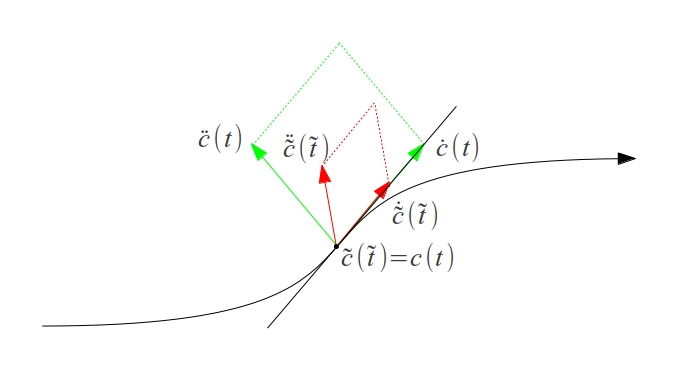
\includegraphics[width=11cm, height=5.5cm]{Bilder/Bsp1.jpg}
\end{figure} 
\end{bsp}

\begin{satz}\label{satz111}
 \(t \mapsto c(t)\) sei Parameterdarstellung einer \(\C^r\)-Kurve im (affinen) \(\IR^n\) mit \(r \ge n\). Dann sind die Ableitungsvektoren\index{Ableitungsvektor} 
 \[
  c_p:= \frac{\dd^p c}{\dd t^p} \, (p=1,\dots, n)
 \]
\uline{nicht} invariant gegenüber Parametertransformationen, jedoch die (punktualen, orientierten) \uline{Schmieg}-\uline{räume}\index{Schmiegraum} (oskulierende Räume, "`osculating spaces"') 
\[
 S_p(t):= c(t) + \langle \langle c_1(t), \dots , c_p(t) \rangle \rangle
\]
Spezialfälle: \\
Tangente \(S_1(t)=c(t) + \langle \langle \dot c(t) \rangle \rangle \) \\
Schmiegebene \( S_2(t) c(t) + \langle \langle \dot c(t), \ddot c(t) \rangle \rangle \)
\end{satz}

\begin{beweis}[von Satz \ref{satz111}]
 Aus \(c = \tilde c \circ \Phi\) folgt nach der Kettenregel
 \begin{align*}
  \dot c &= \dot \Phi \left(\dot{\tilde c} \circ \Phi \right)\\
  \ddot c &= \dot \Phi^2 \left( \ddot{\tilde c} \circ \Phi \right) + Q_2^1 \left( \dot \Phi, \ddot \Phi \right) \cdot \dot {\tilde c}(t)
 \end{align*}
allgemein 
\begin{align*}
 c_p= \dot \Phi^p (\tilde c_p \circ \Phi) + \sum_{k=1}^{p-1} \underbrace{Q_p^k \left( \dot \Phi, \ddot \Phi \right)}_{\text{"`Kettenregelpolynome"'}} \left( \tilde c_k \circ \Phi \right)
\end{align*}
Also hat man die Transformationsformel
\begin{align*}
 \begin{pmatrix}
  c_1 \\
  \vdots \\
  \vdots \\
  c_p
 \end{pmatrix} = \begin{pmatrix}
		  \dot \Phi &0 & \cdots & 0 \\
		  Q_2^1& \dot \Phi^2 & \ddots  & \vdots \\
		  \vdots & \ddots & \ddots &0 \\
		  Q_p^1 & \cdots & Q_p^k & \dot \Phi^p
		 \end{pmatrix} \begin{pmatrix}
				\tilde c_1 \circ \Phi \\
				\vdots \\
				\vdots \\
				\tilde c_p \circ \Phi
			       \end{pmatrix}
\end{align*}
mit einer regulären Transformationsmatrix positiver Determinante. \\
Das zeigt 
\[
 \langle \langle c_1, \dots, c_p \rangle \rangle = \langle \langle \tilde c_1 \circ \Phi, \dots, \tilde c_p \circ \Phi \rangle \rangle
\]
und die weiteren Behauptungen.
\end{beweis}

\begin{bemerkung}
 Die Regularitätsforderung \(\dot c(t) \ne 0\) bedeutet, dass in jedem Punkt die Tangenten als 1-dimensionale Unterräume existieren.
\end{bemerkung}

Die Schmiegräume kann man dazu benutzen, um festzustellen, ob eine Kurve in einem echten affinen Teilraum \(U_p \subset \IR^n\) liegt, in einer Geraden, einer Ebene usw. (affin-invariant!) \\
Zunächst gilt offensichtlich 
\[
 S_1(t) \subseteq S_2(t) \subseteq \dots \subseteq S_n(t) \le p
\]

\begin{satz}\label{satz112} \(\)
 \begin{enumerate}
  \item[a)] Liegt eine \(\C^{p+1}\)-Kurve in einem \(p\)-dimensionalen affinen Unterraum des \(\IR^n\) (\(1 \le p \le n-1 \)), so ist
  \[
   \forall_t \dim S_{p+1}(t) < p+1
  \]
  d.h. der (\(p+1\))-te Schmiegraum degeneriert\index{Schmiegraum!degeneriert}.
  \item[b)] Gilt umgekehrt 
  \[
   \forall_t \dim S_{p+1}(t) = \dim S_p(t) \stackrel{!}{=} p
  \]
  so liegt die Kurve in einem \(p\)-dimensionalen, aber keinem niedriger dimensionalen affinen Unterraum.
 \end{enumerate}
\end{satz}

\begin{anwendung} \(\)
 \begin{enumerate}
  \item Eine \(\C^2\)-Kurve \([c]\) im \(\IR^n\) verläuft genau dann \uline{geradlinig}, wenn \(\forall_t \big(\dot c(t), \ddot c(t)\big) \) linear abhängig ist. \\
  \big["`\(\Rightarrow\)"' nach a), "`\(\Leftarrow\)"' nach b), da \([c]\) regulär\big]
 \end{enumerate}
 \begin{definition}
  Ein (regulärer) Kurvenpunkt \(c(t)\) heißt \uline{Wendepunkt}\index{Wendepunkt} (WP, inflection point), falls \(\big(\dot c(t), \ddot c(t)\big)\) linear abhängig ist.
 \end{definition}
 \begin{enumerate}
  \item[2.] Eine \uline{wendepunktfreie}\index{Wendepunkt!-frei} \(\C^3\)-Kurve \([c]\) im \(\IR^n\) verläuft genau dann \uline{in einer Ebene}, wenn \\ 
  \(\forall_t \big( \dot c(t), \ddot c(t), \dddot c(t) \big) \) linear abhängig ist.
 \end{enumerate}
 \begin{definition}
  Ein \uline{Nicht-Wendepunkt}\index{Nicht-Wendepunkt} \(c(t)\) heißt "`\uline{Henkelpunkt}"'\index{Henkelpunkt} (handle point), wenn \( \big( \dot c(t), \ddot c(t), \dddot c(t) \big) \) linear abhängig ist.
 \end{definition}

\end{anwendung}

\begin{beweis}[von Satz \ref{satz112}] \(\)
 \begin{enumerate}
  \item[a)]
  \begin{align*}
   &\forall_t \quad c(t) = p_0 + \sum_{k=1}^p \lambda_k(t) \cdot a_k \in U_p = p_0 + \hl a_1, \dots, a_p \hr \Rightarrow \\
   &\overset{p+1}{\underset{l=1}\forall} \forall_t \quad c_l(t)= c^{(l)}(t) = \sum_{k=1}^p \lambda_k^{(l)}(t)\cdot a_k \in \hl a_1, \dots, a_p \hr \Rightarrow \\
   & \forall_t \quad \dim S_{p+1}(t) \le p < p
  \end{align*}
  \item[b)] Nach Voraussetzung ist \((c_1, \dots, c_p)(t) \) linear unabhängig, aber \((c_1, \dots, c_{p+1})(t) \) linear abhängig. Es existieren also Funktionen \(t \mapsto \lambda_0(t), \dots, \lambda_{p-1}(t)\) mit 
  \begin{align*}
   c_{p+1} = \sum_{k=1}^p \lambda_{k-1} c_k \text{ bzw. } \uline{(\dot c)^{(p)} = \sum_{k=0}^{p-1} \lambda_k (\dot c)^k} \tag{\(\ast\)}
  \end{align*}
  Die Funktionen sind stetig auf \(I\), denn \((\ast)\) kann nach \(\lambda_0, \dots, \lambda_{p-1}\) aufgelöst werden (Inhomogenes lineares Gleichungssystem mit vollrangiger Koeffizientenmatrix, da \(c_1, \dots, c_p\) linear unabhängig; Einträge und "`rechte Seite"' stetig). \\
  Die Koeffizientenfunktionen \(t \mapsto \dot c^{\,i}(t) \, (i=1,\dots, n)\) genügen also der linearen Differentialgleichung \(p\)-ter Ordnung
  \[
   y^{(p)} = \sum_{k=0}^{p-1} \lambda_k y^{(k)}
  \]
  mit stetigen Koeffizienten.
  für sie existiert ein Fundamentalsystem \(y_1, \dots y_p : I \to \IR\), so dass für jede Lösung gilt
  \[
   y(t)=\sum_{k=1}^p a_k y_k(t)
  \]
  also auch
  \[
   \dot c^{\,i}(t)=\sum_{k=1}^p a_k^i y_k(t)
  \]
  und damit
  \[
   \dot c(t)=\sum_{k=1}^p y_k(t) a_k
  \]
  mit konstanten Vektoren \(a_1, \dots, a_p \in \IR^n\). \\
  Integration liefert \(\forall_{t \in I}\)
  \[
   c(t)= c(t_0) + \sum_{k=1}^p \left(\int_{t_0}^t y_k(\tau) \dd \tau \right) a_k \in c(t_0) + \hl a_1, \dots, a_p \hr =: U_p
  \]
  Es ist schließlich 
  \[
  \uline{\dim U_p =p}
  \] 
  denn aus \(\dim U_p = k < p\) folgt nach a), dass \( \dim S_{k+1} < k+1 \), also auch \(\dim S_p <p\) im Widerspruch zur Voraussetzung.
 \end{enumerate}
  
\end{beweis}

Ab jetzt arbeiten wir im orientierten, \uline{euklidischen} Raum. Hier gibt es zum Glück in jeder Äqui\-va\-lenzklasse von Wegen einen ausgezeichneten Repräsentanten, die \uline{Bogenlängenparametrisierung} (kurz: BLP).

\begin{satz}\label{satz113}
 Sei \(t \mapsto c(t)\) Parameterdarstellung einer \(\C^1\)-Kurve im euklidischen\index{euklidisch} \(\IR^n\). Dann gibt es (bis auf eine additive Konstante) genau eine zulässige Parametertransformation 
 \[
  t \mapsto s(t) = \int|\dot c (t)| \dd t \, [+ s_0]
 \]
 (genannt Bogenlängenfunktion)\index{Bogenlängenfunktion}, so dass in der neuen Bogenlängenparametrisierung\index{Bogenlängenparametrisierung}
 \(
  \overline c = c \circ s^{-1}
 \)
 gilt
 \[
 \uline{|\overline c' | = 1}
 \]
 Die Konstruktion ist unabhängig von der Ausgangsparametrisierung.
\end{satz}

\begin{kin}
In Bogenlängenparametrisierung wird die Kurve mit konstanter Geschwindigkeit \(w = |\overline c'| \equiv 1\) durchlaufen ("`Zeit \(=\) Weg"'). Solche Wege heißen auch normal\index{normal}.
\end{kin}

\begin{beweis}[von Satz \ref{satz113}]
 Für die gesuchte Transformation \(s\) muss wegen 
 \[
 c = \overline c \circ s \Rightarrow |\dot c| = \underbrace{|\overline c' \circ s|}_{= 1} \underbrace{\dot s}_{> 0}
 \]
 gelten: 
 \[
 \dot s = |\dot c|
 \]
Eine Stammfunktion 
 \[
 s = \int |\dot c|
 \]
leistet das Gewünschte, da sie \(\C^1\)-differenzierbar ist, mit 
\(
\dot s = |\dot c| > 0
\)
(wegen der Regularität von \(c\)). \\
 Für eine äquivalente Parametrisierung \(\tilde c\) mit \(c = \tilde c \circ \Phi\) der Kurve erhält man
 \[
  \dot s = |\dot c| = |\dot{\tilde c} \circ \Phi| \underbrace{\dot \Phi}_{> 0} = (\tilde s \circ \Phi) \cdot \dot \Phi
 \]
 also gilt 
 \[s = \tilde s \circ \Phi \, (+ s_0)\] 
 und damit \[\overline c = c \circ s^{-1} = (\tilde c \circ \Phi) \circ (\tilde s \circ \Phi)^{-1} = \tilde c \circ \Phi \circ \Phi^{-1} \circ \tilde s^{-1} = \tilde c \circ \tilde s^{-1} = \overline{\tilde c}\]
\end{beweis}

\begin{bemerkung}
 Mit der Bogenlängenfunktion \(t \mapsto s(t)\) kann man die \uline{Länge}\index{Weg!-länge} eines \(\C^1\)-Wegstücks \\
 \(t \in [a,b] \subset I \mapsto c(t) \in \IR^n\) messen.
 \[
  L_a^b(c) = s(b) - s(a) = \int_a^b |\dot c(t)| \dd t
 \]
 Diese erhält man aus den Längen einbeschriebener Polygonzüge durch Verfeinern und Grenzüber\-gänge. \(\C^1\)-Wege sind rektifizierbar.
\end{bemerkung}

\textbf{\uline{Praktische Berechnung der Bogenlängenparametrisierung}}\index{Bogenlängenparametrisierung!Berechnung} (Schreibweise schlampig): 
\begin{enumerate}
 \item Man berechne \mat{s = s(t) = \int |\dot c(t)| \dd t}
 \item bilde die Umkehrfunktkion \(t=t(s)\)
 \item und bilde \(c(s) = c\big(t(s)\big)\)
\end{enumerate}

\Links

\begin{bsp}
 Ellipse\index{Ellipse} \(t \mapsto c(t) = \vxy{a \cos t}{b \sin t}\) im \(\IR^2\) mit Halbachsen \(0 < a < b\)
 \begin{align*}
  \frac{\dd s}{\dd t}(t) &= |\dot c(t)| = \sqrt{a^2 \sin^2 t + b^2 \cos^2 t} \\
  &= b \cdot \sqrt{1 - \left[1-\left(\frac ab\right)^2\right] \sin^2 t} = b \cdot \sqrt{1-k^2 \sin^2 t} \\
  \Rightarrow s(t) &= b \cdot E(k,t) \, [+ s_0] \quad \text{(Elliptisches Integral 2. Gattung, nicht elementar integrierbar)}
 \end{align*}
 Für einen Kreis (\(a = b = r\)) gilt \(k = 0\) also
 \begin{align*}
  s &= s(t)=r \cdot t \tag {1.}\\
  t &= t(s) = \frac sr \quad \text{also} \tag {2.}\\
  c(s) &= \vxy{r \cos \frac sr}{r \sin \frac sr} \tag {3.}
 \end{align*}
\end{bsp}

\textbf{\uline{Ergebnis}:} \\
Bei Verwendung der Bogenlängenparametrisierung erhält man zwar immer sofort Größen, die invariant gegenüber Parametertransformationen sind.\\
\uline{Aber} meist lässt sie sich nicht explizit bestimmen und ist nur für theoretische Zwecke brauchbar. \\
\uline{Ausweg}: siehe später \\\\
Allgemein zu \uline{Bezeichnungen} (schlampig, aber praktisch)
\begin{center}
\begin{tabular}{c||c|c}
 & bei bel. Par.-Darst. & in BLP \\
 \hline
 \hline
 Parameter & \(t\) [Zeit] & \(s\) [Weg] \\
 \hline
 Parameterdarstellung & \(t \mapsto c(t)\) & \(s \mapsto c(s)\) \\
 \hline
 Ableitungen & \(\dot c, \ddot c, \dddot c, \dots\) [Zeitabl.] & \(c', c'', c''', \dots\) [Abl. nach BL] 
\end{tabular} 
\end{center}
Es gilt 
\[
 \dot c = c' \circ \dot s, \ddot c = c'' \cdot \dot s^2 + c' \ddot s, \dots
\]

\section{Kurven in der euklidischen Ebene $\IR^2$}
siehe Übungen
\section{Kurven im euklidischen Raum $\IR^3$}
\uline{Vorgehensweise} (in jeder Kurven- und Flächentheorie): \\
Konstruktion einer (möglichst invarianten) \uline{Begleitbasis} der Kurve ("`moving frame"'). Ihre \uline{Ableitungs}-\uline{gleichungen} liefern Invarianten für die Kurve, u.a. ihre \uline{Krümmungen}.

\subsection{FRENET-Begleitbasis, Krümmung und Torsion}
Die \uline{Krümmung}\index{Krümmung} einer Raumkurve in Bogenlängenparametrisierung \(s \mapsto c(s)\) soll deren Abweichung vom \uline{geradlinigen Verlauf} messen. Diese wird bestimmt durch die Änderung des (invarianten) Tangenteneinheitsvektors\index{Tangenteneinheitsvektor}
\[
T := c' = \frac{\dd c}{\dd s}
\]
\begin{satz}\label{satz131}
Für die \uline{Krümmung}\index{Krümmung}
\[
 s \mapsto \kappa(s) := |T'(s)| = |c''(s)| \ge 0
\]
einer \(\C^2\)-Kurve in Bogenlängenparametrisierung \(s \mapsto c(s)\) gilt
\begin{enumerate}
 \item[a)] \(\kappa(s_0)=0 \, \Leftrightarrow \,c(s_0)\) Wendepunkt
 \item[b)] \(\kappa \equiv 0 \, \Leftrightarrow\) die Kurve verläuft geradlinig
\end{enumerate}
\end{satz}

\begin{beweis}[von Satz \ref{satz131}] \(\)
 \begin{enumerate}
  \item[a)] \(\kappa(s_0) = 0 \, \Leftrightarrow \, T'(s_0) = 0 {{\color{red}\Leftarrow} \atop \Rightarrow} (c', c'')(s_0) = (T, T')(s_0)\) linear abhängig \\
  \(\Leftrightarrow \, c(s_0)\) ist Wendepunkt \\
  Für die {\color{red}Rückrichtung} wird benötigt: \\
   \[|T|^2 = \langle T,T\rangle = 1 \Rightarrow 2 \langle T',T\rangle = 0 \Rightarrow T' \perp T\] \\
   also \((T,T')(s_0)\) linear abhängig \(\Rightarrow T'(s_0)=0\)
   \item[b)] nach Satz \ref{satz112}, Anwendung 1 oder direkt
   \[
    \kappa \equiv 0 \Leftrightarrow T'= c'' = 0 \Leftrightarrow c(s) = x_0 + s \cdot X
   \]
 \end{enumerate}
\end{beweis}
Noch ein \uline{Test}, ob der Name "`Krümmung"' gerechtfertigt ist: \\
Für einen \uline{Kreis} in Bogenlängenparametrisierung \(s \mapsto c(s) = r \vxyz{\cos \frac sr}{\sin \frac sr}{0}\) im \(\IR^3\) gilt
\begin{align*}
 T(s) &= \vxyz{-\sin \frac sr}{\cos \frac sr}{0} \\
 T'(s) &= \frac 1r \vxyz{-\cos \frac sr}{-\sin \frac sr}{0} \\
 \kappa(s) &= \frac 1r
\end{align*}

\begin{satz}\label{satz132}
 Sei \(s \mapsto c(s)\) Bogenlängenparametrisierung einer \uline{wendepunktfreien} \(\C^2\)-Kurve im orientierten, euklidischen \(\IR^3\). Dann bilden die Vektorfelder
 \begin{align*}
  &s \mapsto T(s) := c'(s) & \text{[Tangentenvektor]} \\
  &s \mapsto H(s) := \frac{T'(s)}{|T'(s)|} & \text{[Hauptnormalenvektor]} \\
  &s \mapsto B(s) := (T \times H)(s) & \text{[Binormalenvektor]}
 \end{align*}\index{Hauptnormalenvektor}\index{Tangentenvektor}\index{Binormalenvektor}
 eine orthonormierte, positiv orientierte \(\C^0\)-Begleitbasis der Kurve, genannt \uline{\textsc{Frenet}-Begleitbasis}\index{Frenet-Begleitbasis}.
\end{satz}

\begin{beweis}[von Satz \ref{satz132}]
 \begin{align*}
  T'\perp T, T' \ne 0 \Rightarrow H \text{ definiert; Rest klar}
 \end{align*}

\end{beweis}

\begin{folgerung}
\begin{figure}[ht]
 \centering
 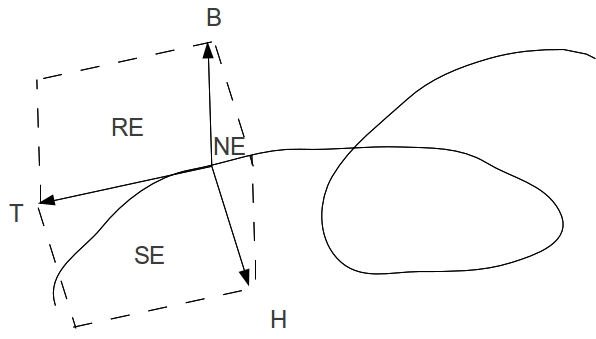
\includegraphics[scale=0.3]{Bilder/Bsp2.jpg}
\end{figure}

 In jedem Kurvenpunkt \(c(s)\) hat man die paarweise orthogonalen \uline{Begleitebenen}\index{Begleitebene}
 \begin{align*}
  &c(s) + \hl T,H \hr(s) \quad \big(\perp B(s)\big) & \text{[Schmiegebene]} \\
  &c(s) + \hl H,B \hr(s) \quad \big(\perp T(s)\big) & \text{[Normalebene]} \\
  &c(s) + \hl B,T \hr(s) \quad \big(\perp H(s)\big) & \text{[rektifizierende Ebene]} 
 \end{align*}\index{Schmiegebene}\index{Normalebene}\index{rektifizierende Ebene}
\end{folgerung}

Die \uline{Torsion}\index{Torsion} (Windung\index{Windung}, \uline{2. Krümmung}\index{Krümmung!2. Krümmung}) einer wendepunktfreien \(\C^3\)-Kurve (\(\Rightarrow (T,H,B) \C^1\)-differen\-zier\-bar) soll deren Abweichung vom ebenen Verlauf messen. Diese wird bestimmt durch die Änder\-ung des Binormalenvektors \(B\) (\(=\) Normalenvektor der Schmiegebene). \\
Wegen \(\begin{Bmatrix}
         B^2 = 1 & \Rightarrow \langle B,B'\rangle = 0  &\Rightarrow B' \perp B \\
         B = T \times H & \Rightarrow B' = \underbrace{T' \times H}_{= 0} + T \times H' &\Rightarrow B' \perp T
        \end{Bmatrix}\) gilt \\
        \(B' = -\tau H\) mit einer \(\C^0\)-Funktion
        \[
         \tau = -\langle B', H\rangle
        \]
        
\begin{satz}\label{satz133}
 Für die durch \(B' = - \tau H\) definierte \uline{Torsion}\index{Torsion} 
 \[
  s \mapsto \tau(s) = - \langle B', H \rangle (s) \stackrel{H \perp B}{=} + \langle H', B \rangle (s) \stackrel{B = T \times H}{=} \det (T,H,H')(s)
 \]
einer \uline{wendepunktfreien} \(\C^3\)-Kurve in Bogenlängenparametrisierung \(s \mapsto c(s)\) gilt
\begin{enumerate}
 \item[a)] \( \tau(s_0) = 0 \Leftrightarrow c(s)\) Henkelpunkt \(\Leftrightarrow \begin{Bmatrix}
                                                                                  (c', c'', c''')(s_0) &\text{linear abhängig} \\
                                                                                  (c',c'') (s_0) & \text{linear unabhängig}
                                                                                 \end{Bmatrix}\)
 \item[b)] \(\tau \equiv 0 \Leftrightarrow\) die Kurve verläuft eben.
\end{enumerate}
\end{satz}

\begin{beweis}[von Satz \ref{satz113}] \(\)
 \begin{enumerate}
  \item[a)] Allgemein gilt
  \begin{align*}
  \langle X \times Y, Z \rangle &= \sum_i (X \times Y)^i Z^i = \sum_{i=1}^3 \det (X,Y,e_i) Z^i \\
  &=\det(X,Y,Z)
  \end{align*}
  Darau folgt
  \begin{align*}
   \tau(s_0) &= \det (T,H,H')(s_0) = \det \left( c', \frac{c''}{\kappa}, \left(\frac{c''}{\kappa}\right)'\right)(s_0) \\
   &= \det \left(c', \frac{c''}{\kappa}, \left(\frac1\kappa\right)' c'' + \frac1\kappa c'''\right)(s_0) = \frac{1}{\kappa^2(s_0)} \det \left(c',c'',c'''\right)(s_0)=0
  \end{align*}
\(\Rightarrow (c', c'', c''')(s_0)\) linear abhängig
  \item[b)] Nach Satz \ref{satz112}, Anwendung 2
 \end{enumerate}
\end{beweis}

\begin{satz}\label{satz134}
 Für die Frenet-Begleitbasis \(s \mapsto (T,H,B)(s)\) einer wendepunktfreien \(\C^3\)-Kurve gelten die Frenetschen \uline{Ableitungsgleichungen}\index{Frenet-Begleitbasis!Ableitungsgleichungen}
 \[\begin{Bmatrix}
  T' &= &&\kappa \cdot H \\
  H' &= &-\kappa T &&+ \tau B \\
  B' &= &&-\tau H
 \end{Bmatrix} \text{bzw.}
 {\vxyz{T}{H}{B}}' = \begin{pmatrix}
                      0 & \kappa & 0 \\
                      -\kappa & 0 & \tau \\
                      0 & -\tau & 0
                     \end{pmatrix} \vxyz{T}{H}{B}
 \]
mit der \(\C^1\)-Krümmung \(s \mapsto \kappa(s) > 0\) und der \(\C^0\)-Torsion \(s \mapsto \tau(s) \).
\end{satz}

\begin{beweis}[von Satz \ref{satz134}] 
Da \((T_1, T_2, T_3) := (T,H,B)\) ein \uline{Orthonormalbasisfeld}\index{Orthonormalbasis!-feld} ist, gilt \(\langle T_i, T_k \rangle = \delta_{ik}\) \\
 \(\Rightarrow \langle T_i', T_k \rangle = -\langle T_k', T_i \rangle\), d.h. die Ableitungsmatrix\index{Ableitungsmatrix} \((\langle T_i', T_k \rangle)_{i,k=1,2,3}\) ist \uline{schiefsymmetrisch}. Damit kann die nach Definition bekannte 1. und 3. Zeile ergänzt werden.
\end{beweis}

\uline{Problem}: Wie berechnet man Begleitbasis, Krümmung und Torsion, wenn man die Bogenlängen\-parametrisierung nicht explizit kennt? \\
\uline{Lösung}: "`Rücktransformation"'

\begin{folgerung}
 Bezüglich einer beliebigen Parametrisierung \(t \mapsto c(t)\) einer wendepunktfreien \(\C^3\)-Kurve gilt
 \begin{align*}
  T &= \frac{\dot c}{|\dot c|} \\
  B &= \frac{\dot c \times \ddot c}{|\dot c \times \ddot c|} \\
  H &= B \times T = \frac{\ddot c - \langle \ddot c, T \rangle T}{|\ddot c - \langle \ddot c, T \rangle T|} \\
  \kappa &= \frac{|\dot c \times \ddot c|}{|\dot c|^3} \\
  \tau &= \frac{\det (\dot c, \ddot c, \dddot c)}{|\dot c \times \ddot c|^2}
 \end{align*}\index{Begleitbasis!Berechnung (unbekannte BLP)}\index{Krümmung!Berechnung (unbekannte BLP)}\index{Torsion!Berechnung (unbekannte BLP)}

\end{folgerung}

\begin{beweis}[der Folgerung]
 \begin{align*}
  &\dot c = c' \cdot \dot s = c' \cdot |\dot c| \Rightarrow T = c' = \frac{\dot c}{|\dot c|} = \frac1w \dot c \\
  &B = T \times H = \frac1\kappa T \times T' = \frac1{w \kappa} T\times \dot T = \frac1{w \kappa} \left(\frac1w \dot c \times \frac{\dd}{\dd t}{\left(\frac1w \dot c\right)}\right) = \frac1{w^3 \kappa} \dot c \times \ddot c = \frac{\dot c \times \ddot c}{|\dot c \times \ddot c|} \\
  &\Rightarrow w^3 \kappa = |\dot c \times \ddot c| \Rightarrow \kappa = \frac{|\dot c \times \ddot c|}{w^3} = \frac{\dot c \times \ddot c}{|\dot c|^3} \\
  &\text{usw. (siehe auch Übungen)}
 \end{align*}

\end{beweis}

\begin{bemerkung}
 Als \uline{Funktionen} sind z.B. \(s \mapsto \kappa(s)\) und \(t \mapsto \kappa(t)\) im Allgemeinen völlig verschieden, obwohl gleich bezeichnet. \\
 Zusammenhang: \(\kappa\big(s(t)\big) = \kappa(t)\) \\
 Analog für \(\tau, T, H, B\).
\end{bemerkung}

\textbf{\uline{Zusatz}:} (später wichtig) \\
Die Basis \((T, H, B)\) erhält man durch Anwendung des Schmidtschen Orthonormalisierungsverfahrens\index{Schmidtsches Orthonormalisierungsverfahren} auf die Basis \((\dot c, \ddot c)\) der Schmiegebene \big(\(\rightarrow (T,H)\)\big) und Ergänzung durch \(B = T \times H\).

\begin{satz}\label{satz135}
 Äquivalent zu den Frenetschen Formeln ist
 \[
  {\vxyz{T}{H}{B}}' = \omega \cdot D \times \vxyz THB
 \]
 mit der \uline{Gesamtkrümmung}\index{Krümmung!Gesamtkrümmung}
 \[
  \omega = \sqrt{\kappa^2 + \tau^2}
 \]
 und dem (normierten) \uline{Darboux-Vektor}\index{Darboux-Vektor}
 \[
  D = \frac1\omega (\tau \cdot T + \kappa \cdot B)
 \]
\end{satz}

\begin{beweis}[von Satz \ref{satz135}]
Nachrechnen unter Verwendung von
\[
 B = T \times H, \quad H = B \times T, \quad T = H \times B
\]
\end{beweis}

\begin{kin} \(\)
\begin{figure}[ht]
 \centering
 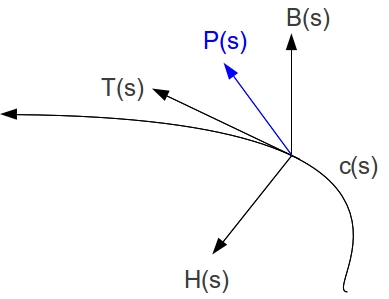
\includegraphics[scale=0.4]{Bilder/Bsp3.jpg}
\end{figure}

 \(s \mapsto c(s)\) beschreibt die Bewegung aus Punkten mit konstanter Geschwindigkeit \(w = |c'| = 1\). Die Bewegung aus starr mit der Begleitbasis \((T_1,T_2,T_3) = (T, H, B)\) verbundenen Punktes
 \[
  P(s) = c(s) + \sum_{i=1}^3 \lambda_i T_i(s) = c(s) + X(s)
 \]
setzt sich zusammen aus einer Translation\index{Translation} (mit der Kurve) und einer Drehung\index{Drehung} um eine momentane Drehachse\index{Drehung!Drehachse}. Für seine Geschwindigkeit gilt
\begin{align*}
 P'(s) &= c'(s) \sum_{i=1}^3 \lambda_i T_i' (s) = c'(s) + \sum_{i=1}^3 \lambda_i w(s) D(s) \times T_i(s) \\
 &=\uline{c'(s) + w(s) D(s) \times X(s)}
\end{align*}
mit der
\begin{itemize}
 \item (vektoriellen) Bahngeschwindigkeit\index{Geschwindigkeit!Bahn-} \(c'(s)\) der Kurve und der 
 \item (vektoriellen) Winkelgeschwindigkeit\index{Geschwindigkeit!Winkel-} \(w\cdot D)(s)\) des Vektors \(X(s) = P(s) - c(s)\) \\
 wobei \(D(s)\) der Einheitsvektor\index{Drehung!Drehachse!Einheitsvektor} der momentanen Drehachse ist \\
 und \(w(s)\)  die skalare Winkelgeschwindigkeit beschreibt
\end{itemize}

\end{kin}

\subsection{Approximierter Kurvenverlauf}
\(s \mapsto c(s)\) sei Bogenlängenparametrisierung einer \(\C^3\)-Kurve mit \(\kappa > 0\). Um einen Parameterwert \(s_0\) (ohne Einschränkung sei \(s_0 = 0\)) besitzt sie die Taylorentwicklung
\[
 c(s) = c(0) + c'(0) s + \frac12 c''(0) s^2 + \frac16 c'''(0) s^3 + \mathcal O(s^3)
\]
Mit \(x_0:= c(0),\, T_0 := T(0), \dots,\, \kappa_0 := \kappa(0), \dots\) folgt wegen \(c' = T,\, c'' = T' = \kappa H,\, c''' = \kappa' H + \kappa (-\kappa T + \tau B)\)

\begin{satz}\label{satz136}
 Eine wendepunktfreie \(\C^3\)-Kurve in Bogenlängenparametrisierung \(s \mapsto c(s)\) im \(\IR^3\) besitzt um \(s = 0\) die Taylorentwicklung\index{Taylorentwicklung}
 \begin{align*}
  c(s) = x_0 &+ \left( s - \frac16 \kappa_0^2 s^3\right) T_0 \\
  &+ \left( \frac12 \kappa_0 s^2 + \frac16 \kappa_0' s^3 \right) H_0 \\
  &+ \left(  \frac16 \kappa_0 \tau_0 s^3\right) B_0 \\
  &+ \mathcal O(s^3)
 \end{align*}
 genannt \uline{lokale kanonische Form}\index{lokale kanonische Form} der Kurve bzgl. des kartesischen Koordinatensystems (\(x_0; T_0, H_0, B_0\)) in der Umgebung von \(s = 0\) . Berücksichtigt man nur Terme niedriger Ordnung, so verhält sie sich in Koordinaten wie
 \[
  s \mapsto \left(s, \frac12 \kappa_0 s^2, \frac16 \kappa_0 \tau_0 s^3 \right)
 \]
\end{satz}

\begin{folgerung}[aus Satz \ref{satz136}] \(\)
 \begin{enumerate}
  \item[a)] Eine Kurve im \(\IR^3\) verläuft in 1. Näherung in ihrer Tangente, in 2. Näherung in ihrer Schmiegebene. Abweichungen davon sind durch Krümmung und Torsion bestimmt.
  \item[b)] Ihre Orthogonalprojektion\index{Orthogonalprojektion}
  \begin{itemize}
   \item in die \uline{Schmiegebene} verhält sich wie eine \uline{(quadratische) Parabel}
   \item in die \uline{Normalebene} verhält sich wie eine \uline{Neil'sche Parabel}
   \item in die \uline{rektifizierende Ebene} verhält sich wie eine \uline{kubusche Parabel}
  \end{itemize}
  Skizze für \(\tau > 0\) \\
  \begin{figure}[ht]
  \begin{minipage}{5cm}
    \centering
   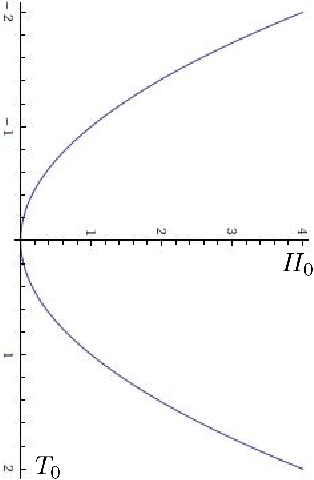
\includegraphics[scale=0.2]{Bilder/T0H0.jpg} \\
   Schmiegebene
  \end{minipage}
  \begin{minipage}{5cm}
   \centering
   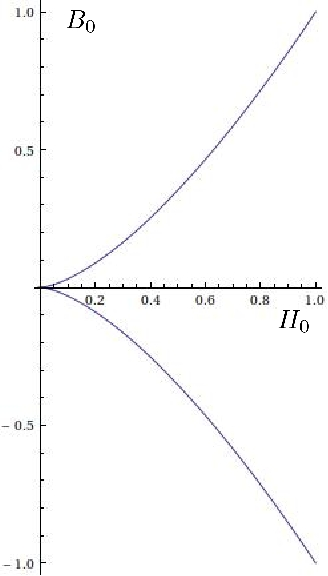
\includegraphics[scale=0.2]{Bilder/H0B0.jpg} \\
   Normalebene
  \end{minipage} 
  \begin{minipage}{5cm}
  \centering
  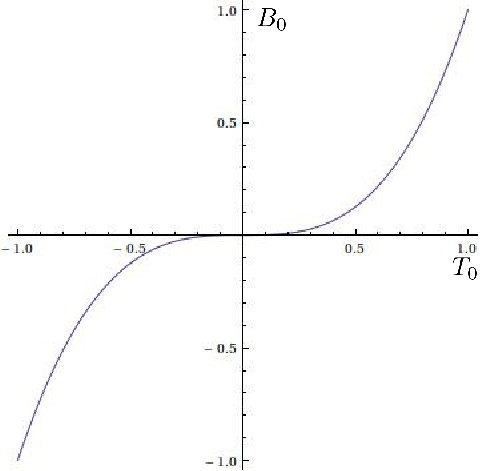
\includegraphics[scale=0.2]{Bilder/T0B0.jpg} \\
  rektifizierende Ebene
  \end{minipage}
   \end{figure} \\
   \begin{figure}[ht]
    \centering
    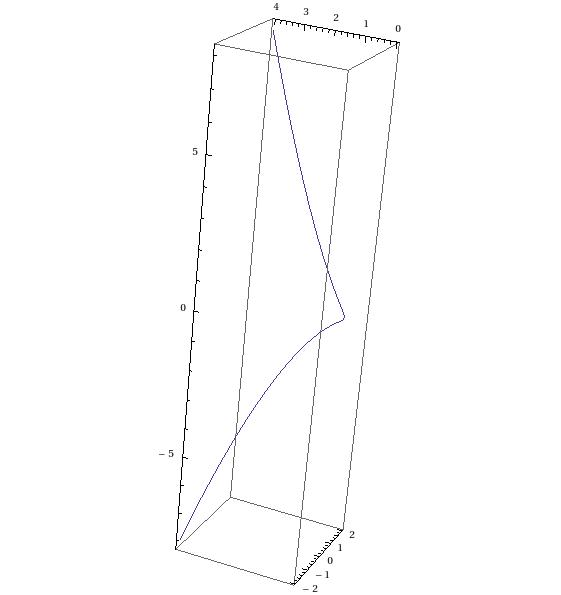
\includegraphics[scale=0.3]{Bilder/Skizze.jpg}
   \end{figure}
  \item[c)] Sie durchdringt ihre Normalebene \(x_0 + \hl H_0, B_0 \hr\) in Richtung von \(T_0\) und ihre Schmiegebene \(x_0 + \hl T_0, H_0 \hr\) für \(\uline{\tau_0 > 0}\) in Richtung von \(B_0\). (Geometrische Bedeutung des \uline{Vorzeichens der Torsion}) \\
  Sie durchdringt die rektifizierende Ebene \(x_0 + \hl B_0, T_0 \hr\) niemals, sondern bleibt auf der Seite, in die \(H_0\) zeigt.
 \end{enumerate}
\end{folgerung}

\subsection{Krümmungskreis und Schmiegkugel (oskulierende Kugel)}\index{Krümmungskreis}\index{Schmiegkugel}
Wir bestimmen alle Kugeln \(K_r(m) = \{ y \in \IR^3 \mid |y-m| = r \}\), die eine vorgegebene Kurve in Bogenlängenparametrisierung \(s \mapsto c(s)\) in einem Punkt \(c(s_0)\) von 2. und 3. Ordnung \uline{berühren}. \\\\
\uline{Berührbedingungen}\index{Berührbedingung} an die Abstandsfunktion \(s \mapsto F(s) := \dd^2 (s) = |c(s) - m|^2\)
\begin{align*}
 F(s_0) &= r^2 &\big(\text{Berührung 0. Ordnung: }c(s_0) \in K_r(m)\big) \\
 \text{zusätzlich } F'(s_0) &= 0 &(\text{Berührung 1. Ordnung}) \\
 \text{zusätzlich } F''(s_0) &= 0 &(\text{Berührung 2. Ordnung}) \\
 \text{zusätzlich } F'''(s_0) &= 0 &(\text{Berührung 3. Ordnung})
\end{align*}

\begin{begruendung} \(\)
\begin{itemize}
 \item Berührung 1. Ordnung \(=\) "`2-punktige Berührung"' 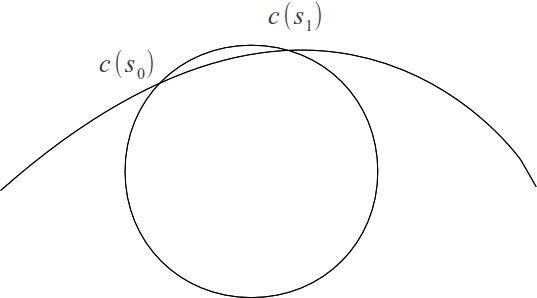
\includegraphics[scale=0.2]{Bilder/Bsp5.jpg} \\
 \(F(s_0) = F(s_1) = r^2 \stackrel{\text{MWS}}{\Rightarrow} \exists_{\overline {s_0} \in \overline{s_0 s_1}} F'(\overline{s_0}) = 0 \) \\
 Grenzübergang \(s_1 \to s_0 (\Rightarrow \overline {s_0} \to s_0)\) liefert \(F'(s_0) = 0\)
 \item Berührung 2. Ordnung \(=\)"`3-punktige Berührung"' \\
 \(F(s_0) = F(s_1) = F(s_2) = r^2 \stackrel{\text{MWS}}{\Rightarrow} \exists_{\overline{s_0}, \overline{s_1}} F'(\overline{s_0}) = F'(\overline{s_1}) = 0 \stackrel{\text{MWS}}{\Rightarrow} \exists_{\overline{\overline{s_0}}} F''(\overline{\overline{s_0}}) = 0\).\\
 Grenzübergang \(s_1, s_2 \to s_0 (\Rightarrow \overline{s_1}, \overline{\overline{s_0}} \to s_0)\) liefert \(F'(s_0) = F''(s_0) = 0\)
\end{itemize}
\end{begruendung}

\uline{Auswertung der Bedingungen}: 
\begin{enumerate}
 \item[(0)] \(F(s_0) = | c(s) - m|^2 = r^2\)
 \item[(1)] \(F'(s_0) = 2 \langle c-m, T \rangle (s_0) = 0\)
 \item[(2)] \(F''(s_0) = 2 \big[ 1 + \kappa \langle c-m, H\rangle \big] (s_0) = 0\)
 \item[(3)] \(F'''(s_0) = 2 \big[ \kappa' \langle c-m, H\rangle + \kappa \langle c-m, -\kappa T + \tau B\rangle \big](s_0) = 0\)
\end{enumerate}

Der Ansatz \(m = c(s_0) + \alpha T(s_0) + \beta H(s_0) + \gamma B(s_0)\) liefert
\begin{align*}
 \alpha &= - \langle c-m, T \rangle(s_0) \\
 \beta &= -\langle c-m, H \rangle(s_0) \\
 \gamma &= -\langle c-m, B\rangle (s_0)
\end{align*}
\begin{enumerate}
 \item[(0)] \(\alpha^2 + \beta^2 + \gamma^2 = r^2\)
 \item[(1)] \(\Rightarrow\) \({\color{red}\alpha = 0}\)
 \item[(2)] \(\Rightarrow\) \({\color{red}\beta = \frac1{\kappa(s_0)}} = \rho(s_0) > 0\) (falls \(\kappa(s_0) > 0\))
 \item[(3)] \((\kappa' \rho + \kappa \tau \gamma)(s_0) = 0\) \(\Rightarrow\) \({\color{red}\gamma = - \frac{\kappa'}{\kappa^2 \tau}(s_0) = \frac{\rho'}{\tau}(s_0)}\) \big[falls \(\tau(s_0) \ne 0\)\big]
\end{enumerate}

\begin{satz}\label{satz137}\(\)
\begin{figure}[ht]
 \centering
 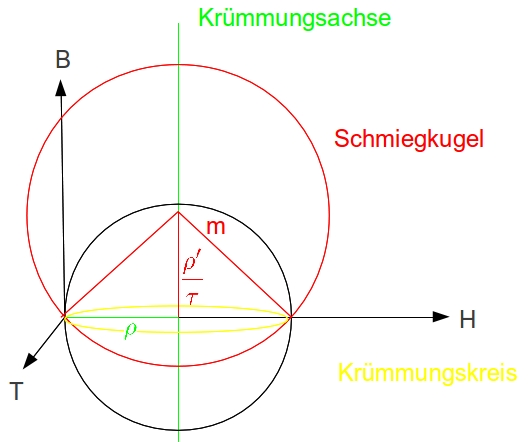
\includegraphics[scale=0.4]{Bilder/Bsp6.jpg}
\end{figure}
\begin{enumerate}
 \item Bei einer \(\C^2\)-Kurve in Bogenlängenparametrisierung \(s \mapsto c(s)\) existiert in einem Nicht-Wendepunkt \(c(s_0)\) (mit \(\kappa(s_0) > 0\)) genau eine 1-parametrige Kugelschar, die dort von 2. Ordnung berührt. Die Mittelpunkte dieser Kugel liegen auf einer Geraden
 \[
  c(s_0) + \rho(s_0) H(s_0) + \hl B(s_0) \hr \quad \left(\text{mit } \rho := \frac1{\kappa}\right)
 \]
 genannt \uline{Krümmungsachse}\index{Krümmungsachse} der Kurve in \(c(s_0)\). \\
 Alle diese Kugeln schneiden die Schmiegebene in einem Kreis mit Mittelpunkt 
 \[\overline m = c(s_0) + \rho (s_0) H(s_0)\] 
 und Radius \[\overline r = \rho(s_0)\quad \big[\text{\uline{Krümmungsradius}}\big]\]
 \index{Krümmungsradius} genannt \uline{Krümmungskreis}\index{Krümmungskreis} der Kurve in \(s_0\).
 \item Bei einer \(\C^3\)-Kurve in Bogenlängenparametrisierung \(s \mapsto c(s)\) existiert in einem Nicht-Henkelpunkt \(c(s_0)\) (mit \(\kappa(s_0) > 0, \tau(s_0) \ne 0\)) genau eine Kugel, die dort \uline{von 3. Ordnung} berührt. Sie besitzt den Mittelpunkt
 \[
  m = c(s_0) + \rho(s_0) H(s_0) + \frac{\rho'}{\tau}(s_0) B(s_0)
 \]
 und den Radius
 \[
  r = \sqrt{\rho^2 + \left(\frac{\rho'}{\tau}\right)^2}(s_0)
 \]
und heißt Schmiegkugel\index{Schmiegkugel} der Korve in \(c(s_0)\).
\end{enumerate}
\end{satz}
